\begin{tikzpicture}[
	node distance=10cm,
	stuff/.style={draw, cloud, cloud ignores aspect, font=\Huge},
	img/.style={text width=3cm, minimum height=3cm},
	arr/.style={->, >={Latex[length=0.4cm]}},
	label/.style={above, fill=white, font=\Huge}
]

\node[stuff] (input) {Feladat};
\node[img, below= 3cm of input] (human) {{\includestandalone[width=\textwidth]{images/human_head}}};
\node[img, right of=human, text width=6cm] (language) {{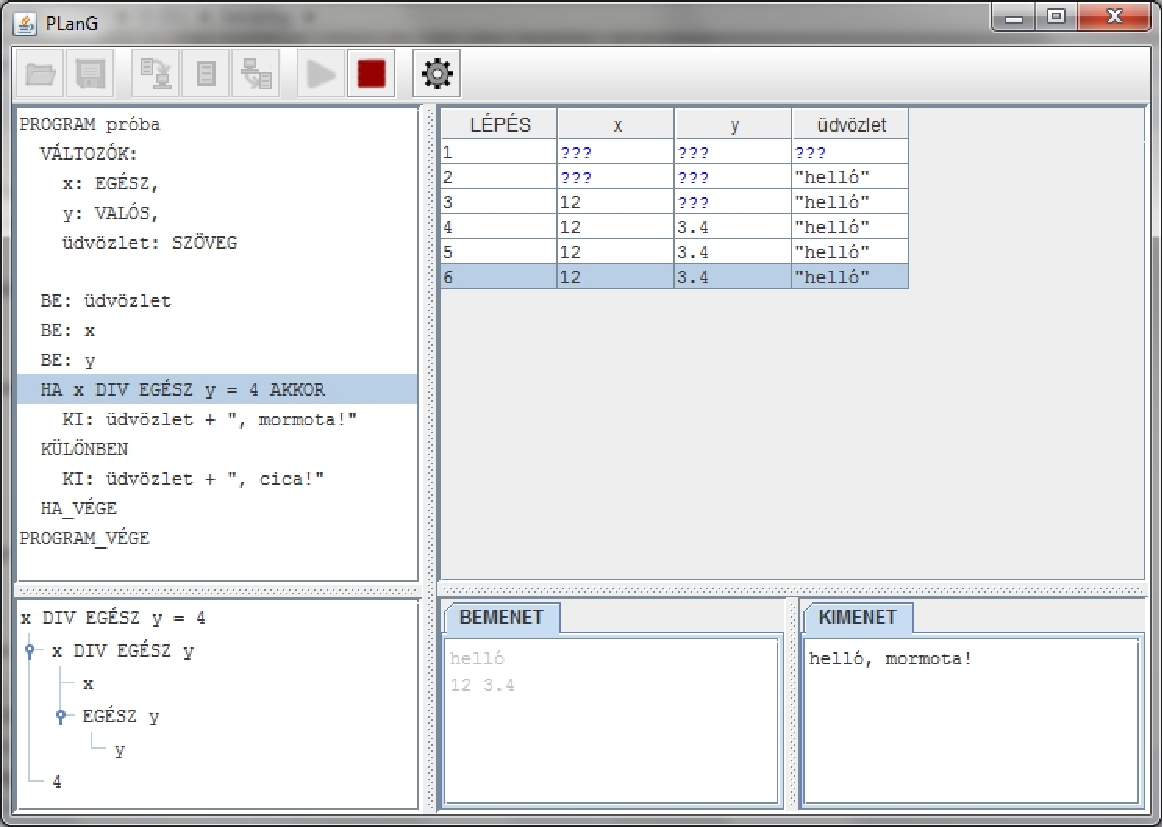
\includegraphics[width=\textwidth]{images/plang.pdf}}};
\node[img, right of=language] (computer) {{\includestandalone[width=\textwidth]{images/computer}}};
\node[stuff, above=3cm of computer] (output) {Megoldás};

\draw[arr] (input) edge (human);
\draw[arr] (human) edge node[label] {algoritmus} (language);
\draw[arr] (language) edge node[label] {program} (computer);
\draw[arr] (computer) edge (output);

\end{tikzpicture}
